\chapter{\textit{Data Warehouse}} 
\label{chap:arquitetura}

Neste capítulo será apresentada a maneira como foi desenvolvido o ambiente de \textit{data warehouse} para armazenamento de métricas de código fonte, sobre o qual esse trabalho busca analisar a eficácia e eficiência no monitoramento de métricas. Serão apresentados anteriormente conceitos teóricos sobre \textit{data warehouse}, para então relacionar seu uso dentro do contexto de métricas. 

\section{Definições e terminologia}

\textit{Data warehouse} é uma base de dados que armazena suas informações de maneira orientada a satisfazer solicitações de tomadas de decisão \cite{chaudhuri1997}. A diferença entre um típico banco de dados transacional e um  \textit{data warehouse}, porém, consiste na maneira como esses dados são armazenados. Em vez de existirem múltiplos ambientes de decisão operando de forma independente, o que com frequência traz informações conflituosas, um \textit{data warehouse} unifica as fontes de informações relevantes, de maneira que a integridade  qualidade dos dados são garantidas. \cite{neeraj_sharma_2011}. Dessa forma, \citeonline{chaudhuri1997} afirma que o ambiente de \textit{Data Warehousing} possibilita que seu usuário realize buscas complexas de maneira mais amigável diretamente em um só ambiente, em vez de acessar informações através de relatórios gerados por especialistas. 

\citeonline{Inmon2002} descreve que o \textit{data warehouse} é uma coleção de dados que tem como característica ser orientada a assunto, integrada, não volátil e temporal. Por orientação a assunto, podemos entender como um foco em algum aspecto específico da organização, como por exemplo as vendas de uma loja. O fato do ambiente ser integrado remete ao fato dele ser alimentado com dados que têm como origem de múltiplas fontes, integrando esses dados de maneira a construir uma única orientação. Como um conjunto não volátil e temporal de dados, é entendido que a informação carregada remete a um determinado momento da aplicação, possibilitando assim acesso a diferentes intervalos de tempo, não havendo como modificá-los atualizando em tempo real. 

São vários os tipos de aplicação aceitos para um \textit{data warehouse}. Algumas delas serão definidas a seguir.


\textbf{OLAP (online analytical processing — processamento analítico on-line)}:
Conjunto de princípios que fornecem uma estrutura dimensional de apoio à decisão \cite{Kimball2002}. As ferramentas OLAP empregam as capacidades de computação distribuída para análises que requerem mais armazenamento e poder de processamento do que pode estar localizado econômica e eficientemente em um \textit{desktop} individual \cite{elmasri_sistemas_2011}. Nestas aplicações dados sumariados e históricos são mais importantes que dados atômicos \cite{hilmer2002}.

\textbf{DSS (decision-support systems — sistemas de apoio à decisão)}:
são sistemas que ajudam os principais tomadores de decisões de uma organização com dados de nível mais alto em decisões complexas e importantes \cite{elmasri_sistemas_2011}. Segundo \citeonline{kimball_data_2008}  os DSSs têm como objetivo tornar a informação de uma organização acessível e consistente, prover uma fonte adaptável e resiliente de informações, e garantir a segurança aos dados para assim ser um sistema base para a tomada de decisão.

\textbf{OLTP (online transaction processing) — processamento on-line de transações}:
bancos de dados tradicionais têm suporte para o OLTP, com suas operações de inserção, atualização e exclusão e também à consulta de dados. \citeonline{neeraj_sharma_2011} explica que sistemas OLTP usam tabelas simples para armazenar dados, estes que são normalizados, para se reduzir a redundância ou até mesmo eliminá-los, buscando sempre a garantia de sua consistência.

\section{Características dos \textit{Data Warehouses}}\label{sec:caract-dw}


\citeonline{elmasri_sistemas_2011} diferencia um \textit{data warehouse} de uma estratégia de multibancos de dados afirmando que o primeiro possui um armazenamento em um modelo multidimensional, assim dados de múltiplas fontes são integrados e processados para tal e sendo assim contrário ao segundo, que oferece acesso a bancos de dados disjuntos e normalmente heterogêneos. A vantagem se nota pela adoção de um padrão de design mais conciso, que pode levar a uma menor complexidade de implantação.

Diferentemente da maioria dos banco de dados transacionais, \textit{data warehouses} costumam apoiar a análise de série temporal e tendência, ambas exigindo mais dados históricos do que geralmente é mantido nos bancos de dados transacionais. É importante notar também que os \textit{data warehouses} são não-voláteis. Sendo assim, suas informações possuem a característica de mudarem de uma forma muito menos frequente, portanto dificilmente seria enquadrada como uma informação em tempo real, e sim como uma de atualização periódica \cite{elmasri_sistemas_2011}.

\citeonline{elmasri_sistemas_2011} ordena as seguintes características diferenciadoras de data warehouses, proveniente da lista original de \citeonline{codd1993providing} sobre OLAP:

\begin{easylist}[itemize]

& Visão conceitual multidimensional.

& Dimensionalidade genérica.

& Dimensões e níveis de agregação ilimitados.

& Operações irrestritas entre dimensões.

& Tratamento dinâmico de matriz esparsa.

& Arquitetura de cliente-servidor.

& Suporte para múltiplos usuários.

& Acessibilidade.

& Transparência.

& Manipulação de dados intuitiva.

& Desempenho de relatório consistente.

& Recurso de relatório flexível.

\end{easylist}

A consulta OLAP difere da consulta do tipo \textit{On-Line Transaction Processing} (OLTP) pelo fato dos seus dados terem passado por um processo de ETL, de modo que sua performance foi melhorada para uma análise mais fácil e rápida, enquanto na consulta do tipo OLTP o sistema foi modelo de modo a capacitar inserções, atualizações e remoções de dados obedecendo regras de normalização. 

A tabela \ref{tab:hilmer} evidencia as principais diferenças entre aplicações OLTP e OLAP extraídas do trabalho de \citeonline{hilmer2002}: 

\begin{table}[!ht]
	\begin{center}
	
	\input{tabelas/tabelasMatheus/hilmer_olap_oltp.ltx} 
	\caption{Diferenças entre OLTP e OLAP extraídas de \citeonline{hilmer2002}}
	\label{tab:hilmer}
	\end{center}
	\end{table}	
	\FloatBarrier	


\subsection{Componentes Básicos de um Data Warehouse}

A Figura \ref{fig:elem-bas-dw} representa a estrutura básica de um \textit{data warehouse} segundo \citeonline{Kimball2002}. Os componentes apresentados serão definidos em seguida.

% @Figure elem-bas-dw
\begin{figure}[h!]
\centering
\includegraphics[keepaspectratio=false,scale=0.71]{figuras/figuras_pedro/elem-bas-dw.eps}
\caption{Elementos básicos de um \textit{data warehouse} extraídos de \citeonline{Kimball2002}}
\label{fig:elem-bas-dw}
\end{figure}
\FloatBarrier

\textbf{Sistemas de Fonte de Dados Operacionais (OSS - \textit{Operational Source Systems})}:
Representa os sistemas que irão prover informações para o \textit{data warehouse}. Seus dados podem ser provenientes de outros sistemas OLTPs, planilhas e etc, que compõem o negócio a ser tratado. Devem ser pensados como fora do \textit{data warehouse} porque há pouco ou nenhum controle sobre o conteúdo e formato dos dados presentes nestes tipos de sistemas legados \cite{Kimball2002}.

\textbf{Área de Preparação dos Dados (DSA - \textit{Data Staging Area})}:
É onde irá ocorrer a possível limpeza e reformatação dos dados antes que sejam carregados no \textit{data warehouse} \cite{elmasri_sistemas_2011}. Essas tarefas caracterizam os passos do processo que consistem na extração, transformação e carga dos dados, conhecido como \textit{Extraction-Transformation-Load} (ETL). Cada um dos passos recebe a seguinte descrição:

\begin{easylist}[itemize]

	& \textbf{Extração: } Primeira etapa do processo de ETL, consiste na leitura e entendimento da fonte 		dos dados, copiando os que são necessário para futuros trabalhos \cite{Kimball2002}.  
	& \textbf{Transformação: } Após a etapa de extração ter sido feita, os dados podem receber diversos tipos de transformações, que incluem correções de conflitos, conversão de formatos, remoção de campos que não são úteis, combinação entre dados de diversas fontes, entre outros \cite{Kimball2002}.
	& \textbf{Carga: } Após ter sido realizado o processo de transformação, os dados já estão prontos para serem carregados no \textit{data warehouse}, tornando possível que todos os dados visualizados após esse processo reflitam a informação que passou pelos processos de extração e transformação \cite{neeraj_sharma_2011}.  

	\end{easylist}


\textbf{Área de Apresentação dos dados (DPA - \textit{Data Presentation Area})}:
Representa a área onde os dados são organizados, armazenados e disponibilizados para consulta direta pelos usuários, autores de relatórios e outras aplicações. Os dados da área de apresentação devem ser dimensionais e atômicos e devem estar de acordo com a arquitetura do \textit{data warehouse} \cite{Kimball2002}.

% @todo explicar Ferramentas de Acesso de dados 

\textbf{Ferramentas de Acesso de dados (DAT - \textit{Data Access Tools})}:

\textbf{Metadados}: Definido como toda a informação no ambiente de \textit{data warehouse} que não são os dados em si \cite{Kimball2002}. Os metadados num ambiente \textit{data warehouse} podem apontar para dados sobre tabelas do sistema, índices, relacionamentos, e etc. \citeonline{kimball1998data} recomenda que a arquitetura de um DW seja orientada a metadados, devido a seu papel crítico de prover informações e parâmetros que permitem que as aplicações executarem suas tarefas com um controle maior sobre os dados provenientes das fontes de dados e outros elementos fundamentais para sua execução.


\section{Modelagem Dimensional}

\citeonline{Kimball2002} afirma que a habilidade de visualizar algo tão abstrato como um conjunto de dados  de maneira concreta e tangível é o segredo da compreensibilidade, de modo que um modelo de dados que se inicia de forma simples tende a ser simples até o final da modelagem, ao contrário de um modelo que já se inicia de forma complicada. Nesse contexto, o modelo dimensional difere em muitos aspectos do modelo normalizado em sua terceira forma normal, também conhecido como modelo entidade-relacionamento. O modelo normalizado contém seus dados divididos em muitas entidades, cada qual identificada como uma tabela, buscando assim evitar redundância entre os dados, sendo eles armazenados em tempo real na medida que forem atualizados. O problema associado a essa solução é a tamanha complexidade adquirida pelos modelos, uma vez que são criadas um número grande de tabelas dificultando assim sua navegação. Em um sentido oposto, a modelagem dimensional resolve esse problema associado à complexidade, uma vez que, mesmo possuindo as mesmas informações que um modelo normalizado, elas estão modeladas de forma que estejam em sintonia com o entendimento do usuário e ao alto desempenho de consultas. 

 
A modelagem multidimensional adotada pelo OLAP é associada de maneira metafórica na literatura a um cubo de dados, cujas arestas definem as dimensões dos dados e as células do cubo contém valores de medida \cite{Kimball2002}. Os cubos de dados têm um foco nas necessidades de negócio e podem ser exemplificados como na Figura \ref{fig:cubo}:

\begin{figure}[h!]
\centering
\includegraphics[keepaspectratio=false,scale=0.60]{figuras/figuras_matheus/cubo.eps}
\caption{Cubo de dados com o fato Venda e dimensões Produto, Funcionário e Tempo}
\label{fig:cubo}
\end{figure}
\FloatBarrier

A Figura \ref{fig:cubo} reflete uma análise em um cubo de dados. As operações possíveis de serem aplicadas a um cubo OLAP são categorizadas a seguir.

\begin{easylist}[itemize]

	& \textbf{\textit{Drill Down:}} \textit{Drilling} em modelagem multidimensional significa ir de um nível hierárquico a outro \cite{ballard_dimensional_2006}. Portanto,  \textit{Drill Down} busca aumentar o nível de detalhamento, partindo de um certo nível de dados para um nível mais detalhado \cite{neeraj_sharma_2011}.  
	& \textbf{\textit{Drill Up:}} Ao contrário da operação \textit{Drill Down}, a \textit{Roll Up} parte de um nível mais detalhado para um nível menos detalhado  \cite{neeraj_sharma_2011}.
	& \textbf{\textit{Slice and Dice:}} Técnica com filosofia parecida à cláusula \textit{where} usada em \textit{SQL}. Permite que sejam criadas restrições na análise dos dados. \cite{valeria2012} 
	& \textbf{\textit{Drill Across:}} Permite que diferentes cubos sejam concatenados \cite{hilmer2002}. Uma operação do tipo \textit{Drill Across} irá simplesmente unir diferentes tabelas fato através de dimensões correspondentes \cite{kimball1998data}. 
	& \textbf{\textit{Pivoting:}} Metaforicamente, significa rotacionar o cubo. Essa técnica altera a ordenação das tabelas dimensionais \cite{hilmer2002}. 
	

	\end{easylist}
	

A Figura \ref{fig:drill}, extraída de \citeonline{neeraj_sharma_2011}, mostra o fluxo percorrido pelo \textit{Drill Down} e pelo \textit{Drill Up} nas consultas OLAP:

\begin{figure}[h!]
\centering
\includegraphics[keepaspectratio=false,scale=0.70]{figuras/figuras_matheus/drill.eps}
\caption{Diferença entre o fluxo seguido pelo Drill Up e pelo Drill Down, extraída de \cite{neeraj_sharma_2011}}
\label{fig:drill}
\end{figure}
\FloatBarrier

\subsection{Tipos de Tabelas do Modelo Multidimensional}

Um modelo dimensional é composto por tabelas fatos e tabelas dimensões, que quando juntas formam o esquema estrela. A tabela fato é a tabela primária no modelo dimensional. O termo \textit{fato} está associado à maneira como ela representa uma medida de negócio \cite{Kimball2002}. Já a tabela dimensão contém descrições textuais dos negócios envolvidos, o que a torna a chave para que o modelo seja utilizável e de fácil entendimento. \citeonline{Kimball2002} faz uma relação direta entre a qualidade do \textit{data warehouse} como um todo e a qualidade e profundidade dos atributos das tabelas dimensão.

\subsection{Esquemas Multidimensionais}

Dois esquemas comuns são o esquema estrela e o esquema floco de neve. O esquema estrela consiste em uma tabela de fatos com uma única tabela para cada dimensão, como pode ser visto na Figura \ref{fig:estrela} \cite{elmasri_sistemas_2011}. O esquema floco de neve é resultado da normalização e expansão das tabelas de dimensão do esquema estrela \cite{ballard_dimensional_2006}. Segundo \citeonline{Kimball2002} o floco de neve não é recomendado em uma ambiente de \textit{data warehouse}, pois quase sempre faz com que a apresentação dos dados ao usuário seja mais complexa, além do impacto negativo que causa sobre o desempenho da navegação.

% O esquema estrela, já definido como a união entre tabelas fato e dimensão, pode ser representado da forma como o exemplo da Figura \ref{fig:estrela} descreve:
 
\begin{figure}[h!]
\centering
\includegraphics[keepaspectratio=false,scale=0.50]{figuras/figuras_matheus/star.eps}
\caption{Esquema estrela extraído de \citeonline{valeria2012}}
\label{fig:estrela}
\end{figure}
\FloatBarrier


\section{Ambiente de \textit{Data Warehousing} para Métricas de Código-Fonte}

A Figura \ref{fig:etl} descreve a arquitetura de um ambiente de \textit{Data Warehousing}. O nível mais baixo, de onde se faz a extração, foi chamado de fonte externa de dados. Para fazer uso de um ambiente de \textit{data warehousing} para armazenamento de métricas, \citeonline{rego_monitoramento_2014} modelou a arquitetura da solução de modo que a fonte externa de dados seriam arquivos contendo métricas de software, como pode ser visto na Figura \ref{fig:arquitetura_solucao}:

\begin{figure}[h!]
\centering
\includegraphics[keepaspectratio=false,scale=0.50]{figuras/figuras_matheus/arquitetura_solucao.eps}
\caption{Arquitetura do ambiente de \textit{Data Warehousing} para métricas de código}
\label{fig:arquitetura_solucao}
\end{figure}
\FloatBarrier

Seguindo a metodologia de \citeonline{Kimball2002} para projetar um \textit{data warehouse}, o projeto de \citeonline{rego_monitoramento_2014} para a solução de \textit{data warehousing} para métricas de código-fonte seguiu os passos da metodologia, definidos em cada sub-seção a seguir.

\subsection{Seleção do Processo de Negócio}

\citeonline{rego_monitoramento_2014} buscou identificar os processos de negócio e seus respectivos requisitos. Assim foram levantados 15 requisitos de negócio, sendo que os oito primeiros se referem a avaliação dos valores percentis das métricas de código-fonte e o restante a avaliação de cenários de limpeza e taxa de aproveitamento de oportunidades de melhoria de código-fonte. Os requisitos levantados por \citeonline{rego_monitoramento_2014} foram os seguintes:

\begin{easylist}[itemize]

	& \textbf{Requisito 1:} Visualizar o intervalo qualitativo obtido para cada métrica de código-fonte em uma determinada release do projeto para a configuração Open JDK8 Metrics.
	 
	& \textbf{Requisito 2:} Comparar o intervalo qualitativo obtido para cada métrica de código-fonte ao longo de todas as releases de um projeto para a configuração Open JDK8 Metrics 

	& \textbf{Requisito 3:} Visualizar o o valor pecentil obtida para cada métrica de código-fonte em uma determinada release do projeto para a configuração Open JDK8 Metrics
	
	& \textbf{Requisito 4:} Comparar o o valor pecentil a para cada métrica de código-fonte ao longo de todas as releases para a configuração Open JDK8 Metrics.
	
	& \textbf{Requisito 5:} Visualizar o intervalo qualitativo obtido para cada métrica de código-fonte em uma determinada release do projeto para a configuração Tomcat Metrics.
	
	& \textbf{Requisito 6:} Comparar o intervalo qualitativo obtido para cada métrica de código-fonte ao longo de todas as releases de um projeto para a configuração Tomcat Metrics
	
	& \textbf{Requisito 7:} Visualizar a medida obtida para cada métrica de código-fonte em uma determinada release do projeto para a configuração Tomcat Metrics
	
	& \textbf{Requisito 8:} Comparar o valor percentil obtido para cada métrica de código-fonte ao longo de todas as releases para a configuração Tomcat Metrics
	
	& \textbf{Requisito 9:} Visualizar a quantidade de cenários de limpeza identificados por tipo de cenários de limpeza de código-fonte em cada classe ao longo de cada release de um projeto.
	
	& \textbf{Requisito 10:} Comparar a quantidade de cenários de limpeza por tipo de cenários de limpeza de código-fonte em uma release de um projeto.
	
	& \textbf{Requisito 11:} Visualizar o total de cenários de limpeza em uma determinada release de um projeto.
	
	& \textbf{Requisito 12:} Visualizar cada uma das classes com um determinado cenário de limpeza de código-fonte ao longo das releases do projeto.
	
	& \textbf{Requisito 13:} Visualizar as 10 classes de um projeto com menor número de cenários de limpeza identificados.
	
	& \textbf{Requisito 14:} Visualizar as 10 classes de um projeto com maior número de cenários de limpeza identificados.
	
	& \textbf{Requisito 15:} Acompanhar a Taxa de Aproveitamento de Oportunidades de Melhoria de Código-Fonte que é a divisão do total de cenários de limpeza identificados em uma release e o o número total de classes da mesma release de um projeto.

	\end{easylist}


\subsection{Verificação da Periodicidade de Coleta de Dados}

A identificação da periodicidade de coleta dos dados é essencial para que esta seja
realizada de maneira correta, além de viabilizar a agregação dos dados em níveis ou
hierarquias \cite{rego_monitoramento_2014}. Assim a periodicidade foi identificada como as \textit{releases} do software.

\subsection{Identificação dos Fatos e das Dimensões}
	
Para alcançar os requisitos definidos, \citeonline{rego_monitoramento_2014} identificou os seguintes fatos e dimensões no contexto de monitoramento de métricas:

\begin{table}[!ht]
	\begin{center}
	
	\input{tabelas/tabelasMatheus/fatos-dimensoes.ltx} 
	\caption{Fatos e dimensões identificadas por \citeonline{rego_monitoramento_2014}}
	\label{tab:fatos-dimensoes}
	\end{center}
	\end{table}	
	\FloatBarrier


A partir da identificação de fatos e dimensões expostos na Tabela \ref{tab:fatos-dimensoes},  \citeonline{rego_monitoramento_2014} traduziu esses elementos em tabelas fato e tabelas dimensão. O resultado disso pode ser verificado na tabela \ref{tab:tabelas-fatos-dimensoes}:

\begin{table}[!ht]
	\begin{center}
	
	\input{tabelas/tabelasMatheus/tabelas-fatos-tabelas-dimensoes.ltx} 
	\caption{Tabelas fatos e tabelas dimensões elaboradas por \citeonline{rego_monitoramento_2014}}
	\label{tab:tabelas-fatos-dimensoes}
	\end{center}
	\end{table}	
	\FloatBarrier


Utilizando a ferramenta \textit{MySql Workbench}, \citeonline{rego_monitoramento_2014} elaborou o seguinte modelo físico baseado nos fatos e dimensões já identificados:

\begin{figure}[h!]
\centering
\includegraphics[keepaspectratio=false,scale=0.50]{figuras/figuras_matheus/modelo-dw-baufaker.eps}
\caption{Projeto físico do \textit{Data Warehouse} extraído de \citeonline{rego_monitoramento_2014}}
\label{fig:arquitetura_solucao}
\end{figure}
\FloatBarrier

Com o intuito de representar os dados que representam os próprios dados dos processos de negócio, \citeonline{rego_monitoramento_2014} criou uma área de metadados visando facilitar o processo de \textit{Extraction-Transformation-Load}, sendo essa uma vantagem apresentada por \cite{Kimball2002}. A área de metadados desenvolvida possui as seguintes tabelas:

\begin{easylist}[itemize]

	& \textbf{\textit{Meta\_Metric\_Ranges:}} Contém cada configuração de intervalo qualitativo para cada métrica de código fonte.
	& \textbf{\textit{Meta\_Scenario:}} Contém os cenários de limpeza de código e suas recomendações.
	& \textbf{\textit{Meta\_Metric\_Ranges\_Meta\_Scenario:}} Como a cardinalidade entre as tabelas \textit{Meta\_Scenario} e \textit{Meta\_Metric\_Ranges} seria de \textit{n} para \textit{n}, essa tabela foi criada contendo os registros únicos dessas duas tabelas.
	
	\end{easylist}

A Figura \ref{fig:metadados} retrata o ambiente de metadados criado:

\begin{figure}[h!]
\centering
\includegraphics[keepaspectratio=false,scale=0.6]{figuras/figuras_matheus/metadados-baufaker.eps}
\caption{Projeto físico do \textit{Data Warehouse} extraído de \citeonline{rego_monitoramento_2014}}
\label{fig:metadados}
\end{figure}
\FloatBarrier



\section{Considerações Finais do Capítulo}

Nesse capítulo foi apresentada a solução proposta no trabalho de \citeonline{rego_monitoramento_2014}, bem como a base teórica para se chegar nessa solução. No próximo capítulo será apresentado o projeto de estudo de caso que irá visar a análise da eficácia e eficiência da solução proposta nesse capítulo.
